\documentclass[12pt]{article}
\usepackage[margin=1 in]{geometry}
\usepackage{graphicx}
\usepackage{float}
\usepackage{booktabs}
\usepackage{siunitx}
\usepackage{amsmath}
\usepackage{amssymb}
\usepackage{pgfplots}
\pgfplotsset{compat=1.17}

\title{Lab 11: Op-Amp Circuits, Design and Limitations}
\author{Sean Balbale}
\date{November 19th, 2024}
\setlength{\parindent}{0in}

\begin{document}

\begin{titlepage}
  \begin{center}
    \vspace*{1in}

    \Huge
    \textbf{Lab 11}

    \LARGE
    Op-Amp Circuits, Design and Limitations

    \vspace{3 in}

    \textbf{Student Name:} Sean Balbale
    \\ \textbf{Instructor:} Dr. Iman Salama
    \\ \textbf{Lab Partner Name:} Krish Gupta
    \\ \textbf{Date:} November 19, 2024

    \vfill

  \end{center}
\end{titlepage}

\newpage

\section{Introduction}
Operational amplifiers (op-amps) serve as fundamental components in numerous
sensing and measurement applications, particularly in the amplification and
filtering of signals. In biomedical contexts, such as ECG signal acquisition,
op-amps are critical for enhancing small signal magnitudes, rejecting
common-mode signals, and filtering out extraneous noise at high and low
frequencies. This laboratory exercise investigated an active high-pass filter
configuration utilizing the LT1490 operational amplifier. This setup aimed to
replicate prior theoretical analysis performed in LTSpice by assembling and
testing an active filter to observe its in-band gain, time constant, cutoff
frequency, and response characteristics. By constructing this high-pass filter
circuit, the lab provided an opportunity to evaluate practical op-amp
applications and assess discrepancies between theoretical and experimental data,
particularly in the filter's performance across varying frequencies.

\section{Results}
% \begin{figure}[H]
%   \centering
%   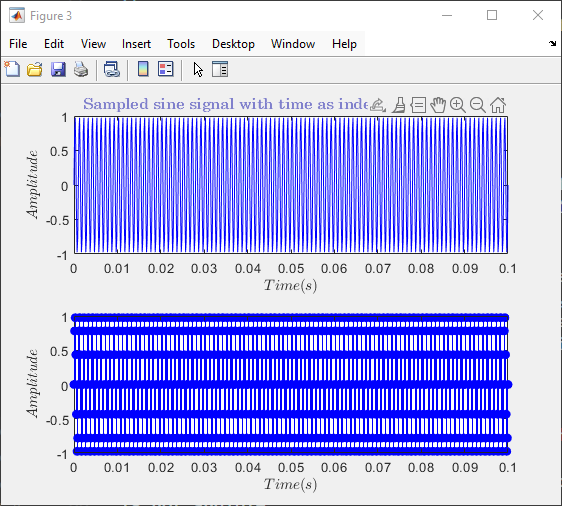
\includegraphics[width=0.3\textwidth]{fig 1f 7000.png}\hfill
%   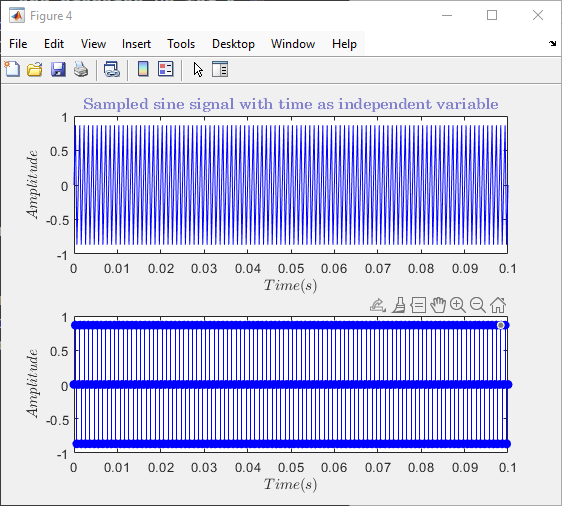
\includegraphics[width=0.3\textwidth]{fig 1f 3000.png}\hfill
%   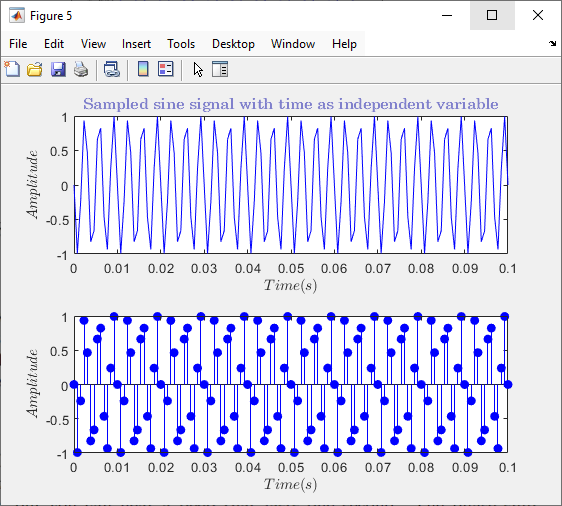
\includegraphics[width=0.3\textwidth]{fig 1f 1300.png}
%   \caption{Sinusoidal with $f_s$ = 7 kHz, 3 kHz, and 1.3 kHz}
%   \label{fig:fig3}
% % \end{figure}
\begin{figure}[H]
  \centering
  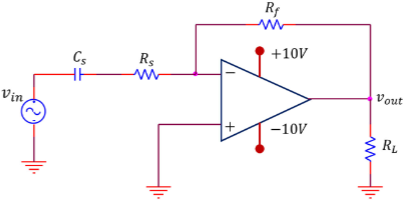
\includegraphics[width=0.5\textwidth]{photos/First Order Active High Pass Filter.png}
  \caption{First Order Active High Pass Filter}
  \label{fig:FirstOrderActiveHighPassFilter}
\end{figure}

The active high-pass filter circuit was constructed as shown in Figure \ref{fig:FirstOrderActiveHighPassFilter}.
It used an LT1490 operational amplifier with three resistors and one capacitor.
The resistor values were $R_s = 98.1 \; k\Omega$, $R_f = 198.6 \; k\Omega$, and $R_L = 9.85 \; k\Omega$.
The capacitor value was $C_s = 10.9 \text{ nF}$. The circuit was assembled on a breadboard
and connected to a function generator and oscilloscope (Figure \ref{fig:filteronbreadboard}).

\begin{figure}[H]
  \centering
  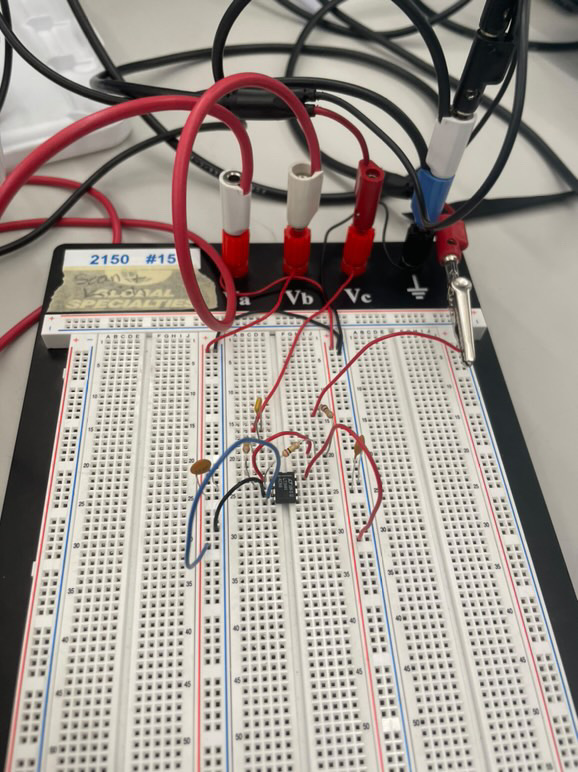
\includegraphics[width=0.5\textwidth]{photos/Circuit Photo 2.jpg}
  \caption{High Pass Filter on Breadboard}
  \label{fig:filteronbreadboard}
\end{figure}

The theoretical in-band gain of the high-pass filter $(H(\omega))$ was
calculated using the following equation:
\[
  H(\omega) = \frac{R_f}{R_s} = \frac{198.6 k\Omega}{98.1 k\Omega} = 2.02
\]
The cutoff frequency of the high-pass filter $(f_c)$ was calculated using the following equation:
\[
  f_c = \frac{1}{2\pi R_s C_s} = \frac{1}{2\pi \cdot 98.1 k\Omega \cdot 10.9 nF} = 148.8 \text{ Hz}
\]
The time constant of the high-pass filter $(\tau)$ was calculated
using the following equation:
\[
  \tau = \frac{1}{2 \pi f_c} = \frac{1}{2 \pi \cdot 148.8 Hz} = 1.07 \text{ ms}
\]
Finally, the cuttoff angular frequency of the high-pass filter $(\omega_c)$ was calculated using the
following equation:
\[
  \omega_c = 2 \pi f_c = 2 \pi \cdot 148.8 \text{ Hz} = 935.5 \text{ rad/s}
\]

The function generator was configured to produce a sine wave with an amplitude of 0.2V peak to peak
with a frequency of of 5 kHz.
The oscilloscope was connected to the output of the high-pass filter to measure the input and
output signals. The input voltage was measured to be 221 mV peak to peak and the output voltage was
measured to be 440 mV peak to peak. The in-band gain was calculated to be:
\[
  H(\omega) = \frac{V_{out}}{V_{in}} = \frac{440 mV}{221 mV} = 1.991 \approx 2.02
\]
The transfer function of the circuit was measured by varying the frequency of the input signal
and measuring the output signal. The results are shown in Table \ref{tab:transferfunction}.
\begin{table}[H]
  \centering
  \begin{tabular}{|l|l|}
    \hline
    f\_c (Hz) & gain  \\ \hline
    10        & 0.25  \\ \hline
    100       & 1.11  \\ \hline
    1000      & 2     \\ \hline
    10000     & 2.09  \\ \hline
    100000    & 0.63  \\ \hline
    1000000   & 0.145 \\ \hline
    10000000  & 0.145 \\ \hline
  \end{tabular}
  \caption{Transfer Function of High Pass Filter}
  \label{tab:transferfunction}
\end{table}

The transfer function was plotted on a Bode plot (Figure \ref{fig:transferfunctionplot}).
\begin{figure}[H]
  \centering
  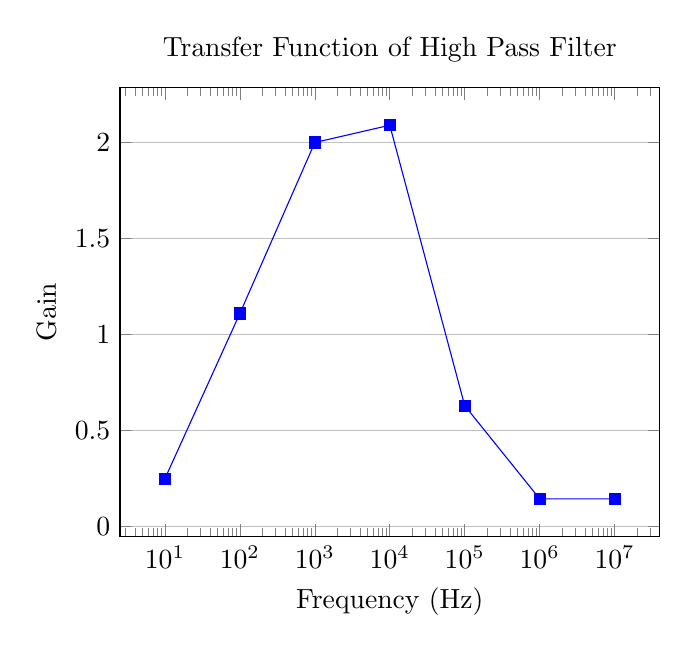
\begin{tikzpicture}
    \begin{axis}[
        xlabel={Frequency (Hz)},
        ylabel={Gain},
        xmode=log,
        log basis x={10},
        grid=both,
        minor x grid style={transparent},
        major x grid style={transparent},
        title={Transfer Function of High Pass Filter}
      ]
      \addplot[
        color=blue,
        mark=square*
      ] coordinates {
        (10, 0.25)
        (100, 1.11)
        (1000, 2)
        (10000, 2.09)
        (100000, 0.63)
        (1000000, 0.145)
        (10000000, 0.145)
      };
    \end{axis}
  \end{tikzpicture}
  \caption{Transfer Function of High Pass Filter}
  \label{fig:transferfunctionplot}
\end{figure}

The gain gets smaller at higher frequencies, which is expected for a
high-pass filter. This is because the op-amp has a limited bandwidth
and cannot amplify signals at high frequencies.
\newline

Now the circuit is connected to a funciton generator that produces a square
wave with a frequency of 50 Hz and amplitude of 0.5 V. The output signal can be
seen in Figure \ref{fig:squarewaveoutput1}.

\begin{figure}[H]
  \centering
  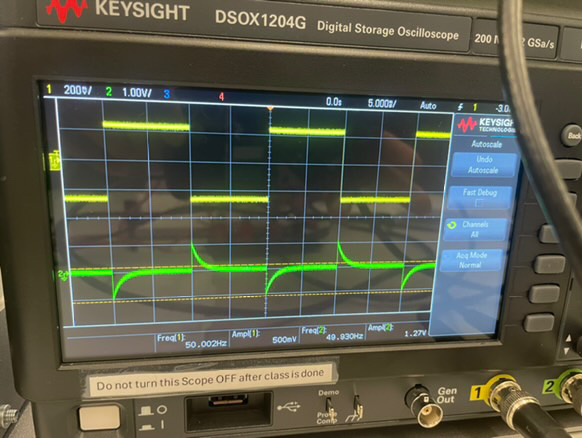
\includegraphics[width=0.5\textwidth]{photos/Oscilloscope 2.jpg}
  \caption{Square Wave Output 50 Hz Input}
  \label{fig:squarewaveoutput1}
\end{figure}

The weird shape of the output signal in Figure \ref{fig:squarewaveoutput1} is due to
the fact that the capacitor
in the high-pass filter is charging and discharging. This causes
the output signal to have a slow rise and fall time. When the frequency
of the input signal is increased to 2 kHz, the output signal can be seen in
Figure \ref{fig:squarewaveoutput2}.
\newline

\begin{figure}[H]
  \centering
  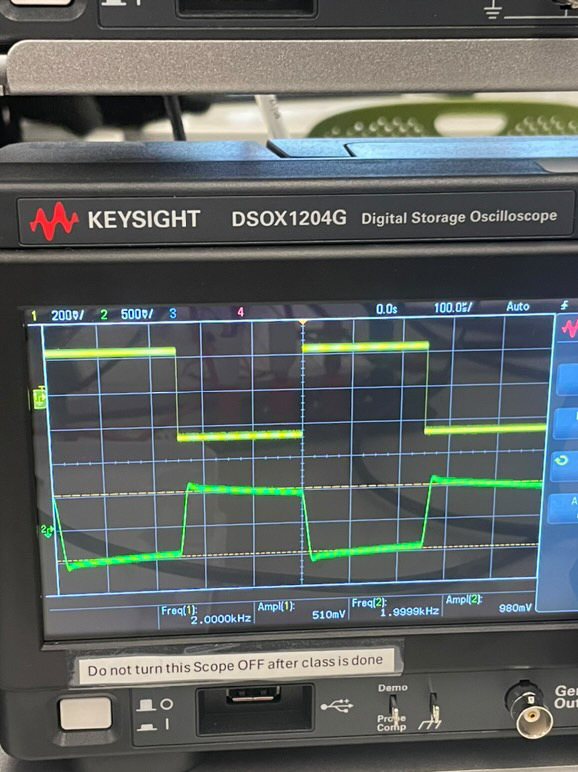
\includegraphics[width=0.5\textwidth]{photos/Oscilloscope 3.jpg}
  \caption{Square Wave Output 2 kHz Input}
  \label{fig:squarewaveoutput2}
\end{figure}

Here, the output signal is a square wave with a faster rise
and fall time. Thus it looks closer to a square wave than the
output signal in Figure \ref{fig:squarewaveoutput1}.

\section{Discussion and Conclusion}
The experiment successfully demonstrated the design, assembly, and testing of an
active high-pass filter using an LT1490 operational amplifier. The high-pass
filter achieved the expected frequency-dependent behavior, with a measured
in-band gain and cutoff frequency that closely matched theoretical calculations.
The cutoff frequency was calculated to be approximately 148.8 Hz, and
experimental measurements supported this value, with a clear gain reduction
observed beyond the cutoff point.
\newline

Results from the Bode plot showed that the filter maintained a consistent gain
in the passband while gradually attenuating signals as frequencies approached
and exceeded the cutoff. At higher frequencies, gain decreased further due to
the op-amp's finite bandwidth, an expected limitation for this component.
\newline

The filter's response to square wave inputs at different frequencies
illustrated its behavior in the time domain, where the capacitor charging and
discharging caused distinctive wave-shaping effects. At low frequencies, the
output signal exhibited rounded edges, whereas, at higher frequencies, the
output signal retained a more defined square shape. This outcome aligns with
high-pass filter principles, as the circuit more effectively transmitted
higher-frequency components.
\newline

In conclusion, the lab provided hands-on insight into op-amp-based filter
design, confirming theoretical expectations and highlighting practical
considerations such as component tolerances and frequency limitations of the
op-amp. The results affirm the utility of high-pass filters in applications that
require selective attenuation of low-frequency noise, such as biomedical signal
processing.
\section{References}
[1] Dr. Iman Salama. “Lab 11 – Op-Amp Circuits, Design and Limitations” Northeastern University. 11 November 2024.

\end{document}
